\section{The classical Black Hole Area Theorem}
\label{sec:classical-bh-area}

Our statement of the original Black Hole area theorem comes from \cite{wald2010general} (theorem \(12.2.6\)):
\begin{theorem}[Black Hole Area Theorem]
	\label{th:classical-bh-area}
	Let \((M, g_{\mu\nu})\) be a strongly asymptotically predictable spacetime satisfying \(R_{\mu\nu}U^{\mu}U^{\nu} \ge 0\) for all null vectors \(U^{\mu}\) (\emph{null convergence condition}). Let \(\Sigma_1\) and \(\Sigma_2\) be spacelike Cauchy surfaces for the globally hyperbolic region \(\tilde{V}\) such that \(\Sigma_2 \subset I^+(\Sigma_1)\), and given \(H\) the event horizon we define
	\[
	\mathscr{H}_1 = H \cap \Sigma_1, \quad \quad \mathscr{H}_2 = H \cap \Sigma_2.
	\]
	Then the area of \(\mathscr{H}_2\) is greater or equal than the area of \(\mathscr{H}_1\).
\end{theorem}

\begin{proof}
	This theorem is usually proven by showing, through a reductio ad absurdum, that the expansion \(\theta\) of the null geodesic generators of \(H\) is everywhere non-negative. Here we wish to follow a slightly different path, inspired by the index form methods, that makes use of another object, defined in section \ref{sec:submanifolds}: the mean curvature.
	
	Let \(\Sigma_1\) be any Cauchy hypersurface for \(\tilde{V}\) through a generic point \(p\in H\), and call \(\mathscr{H}_1 = H \cap \Sigma_1\), as above. Finally refer to \(\mathrm{H}^{\mu}\) as the mean normal curvature of \(\mathscr{H}_1\).
	The core of the proof is showing that, for the tangent field \(U^{\mu}\) of the null generators of the horizon \(H\), it holds everywhere that:
	\begin{equation}
	\label{eq:exp-null-generators}
		\mathrm{H}^{\mu}U_{\mu} \ge 0.
	\end{equation}
	By contradiction, suppose instead that \(\mathrm{H}^{\mu}U_{\mu} < 0\) at \(p\in \mathscr{H}_1\). We then want to extend the function \(\mathrm{H}^{\mu}U_{\mu}\) in a continuous way on \(\Sigma_1\) (at least in a neighborhood of \(\mathscr{H}_1\)). 
	\noindent
	In order to do that, take any deformation of \(\mathscr{H}_1\) outward on \(\Sigma_1\), say \(\mathscr{H}_1'\) and call \(K\) the closed region in \(\Sigma_1\) between \(\mathscr{H}_1\) and \(\mathscr{H}_1'\); the boundary of its future \(\partial J^+(K)\) is a null hypersurface of codimension \(1\), and hence comes with its own null generators, with tangent field \(U'^{\mu}\) (see figure \ref{fig:extension-area-theorem}). This allows us to define the function in \(p' \in\mathscr{H}_1'\) as simply the contraction 
	\(\mathrm{H}'^{\mu}U'_{\mu}\) (with \(\mathrm{H}'^{\mu}\) mean normal curvature of \(\mathscr{H}_1'\)). Different deformations of \(\mathscr{H}_1\) may give different extensions, but that's not important, since we only need that there exists one so that the extension is smooth.
	
	\begin{figure}
		\centering
		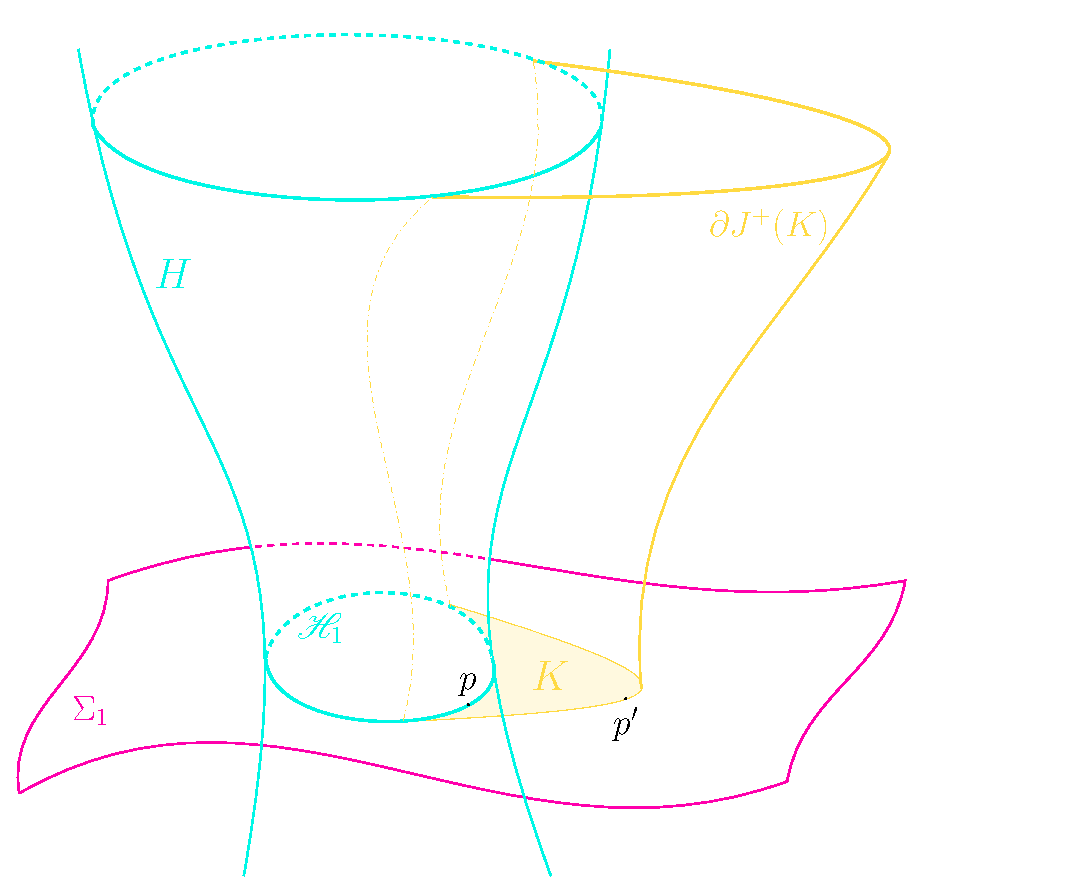
\includegraphics[scale=0.8]{Immagini/extension-area-theorem/extension-area-theorem.pdf}
		\caption[]{schematic representation about how to construct the extension of the function \(\mathrm{H}^{\mu}U_{\mu}\).}
		\label{fig:extension-area-theorem}
	\end{figure}
	\begin{SCfigure}
		\centering
		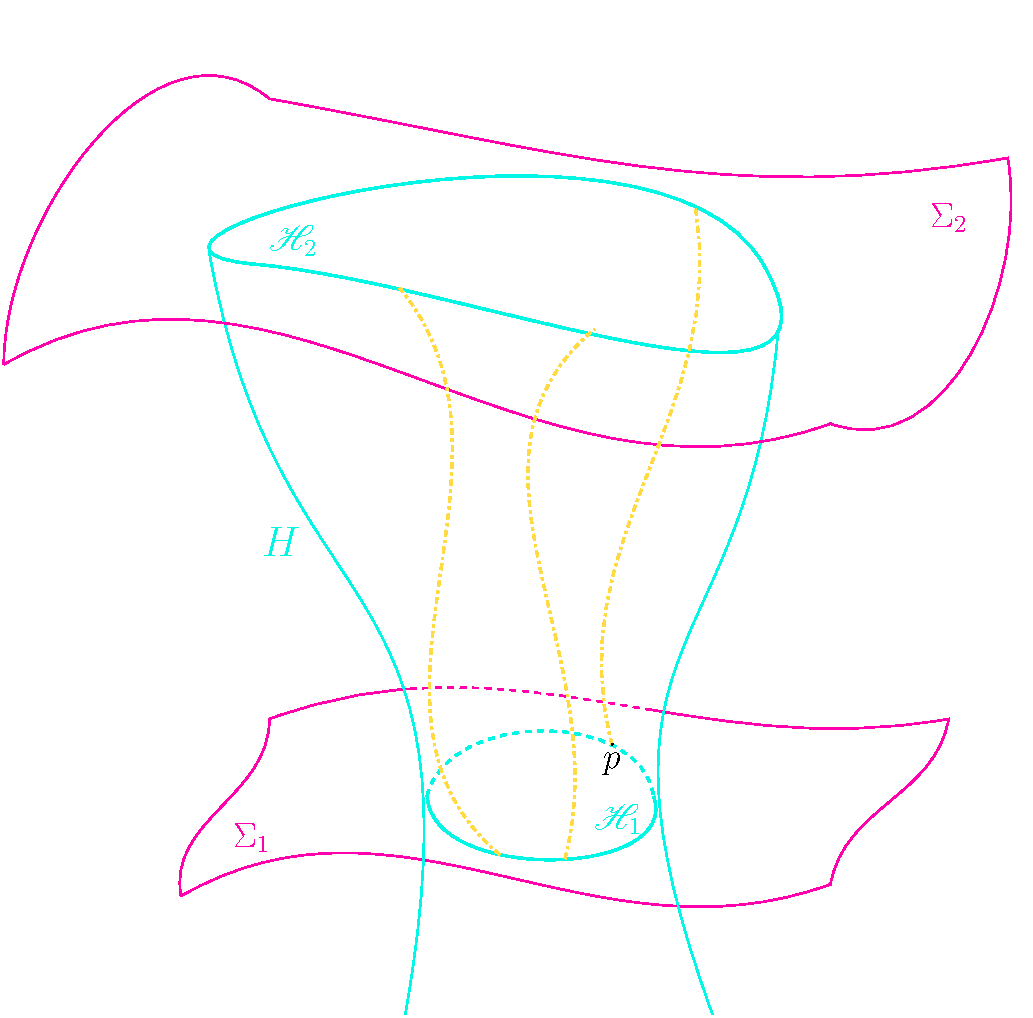
\includegraphics[scale=0.37]{Immagini/flow-generators/flow-generators.pdf}
		\caption[]{the flow along the null generators of the horizon maps \(\mathscr{H}_1\) into (a part of) \(\mathscr{H}_2\).}
		\label{fig:flow-generators}
	\end{SCfigure}
	Given that extension, for continuity it exists a neighborhood of \(p\) in which \(\mathrm{H}^{\mu}U_{\mu}(p) < 0\); we can pick a deformation \(\mathscr{H}_1\) outward on \(\Sigma_1\), to \(\mathscr{H}_1'\), such that
	\[
	\begin{cases}
	J^-(\mathscr{I}^+) \cap \mathscr{H}_1' \neq \emptyset; \\
	\mathrm{H}'^{\mu}U'_{\mu} < 0 \text{ everywhere on } 	J^-(\mathscr{I}^+) \cap \mathscr{H}_1'.
	\end{cases}
	\]
	Pick now a point \(q \in \mathscr{I}^+ \cap \partial J^+(K)\):  
	% (\VS{This exists for sth similar to 12.2.6 of Wald})
	the null geodesic generator through \(q\) will meet \(\mathscr{H}_1'\) orthogonally because of \ref{prop:global-existence} and \ref{prop:perp-critical-gamma}; however, in \(p' = \gamma \cap \mathscr{H}_1'\), \(U'_{\mu}\mathrm{H}'^{\mu} < 0\), so by proposition \ref{prop:fp-criteria} we know that a focal point to \(\mathscr{H}_1'\) must develop on \(\gamma\) before reaching \(q\). In fact, it is enough to choose \(f = 1 - \frac{\lambda}{\ell}\), with \(\lambda\) affine parameter such that:
	\[
	\begin{cases}
	\hat{\mathrm{H}}'^{\mu}U'_{\mu} = 1 \\
	\gamma(\lambda = 0) = p' \\
	\ell \ge  \frac{1}{\vert U'_{\mu}\mathrm{H}'^{\mu} \vert}
	\end{cases}
	\]
	and 
	{\small
	\[
	\int_{0}^{\ell} \big((n -2)(\nabla_{U'}f)^2 - f^2R_{\mu\nu}U'^{\mu}U'^{\nu} \big)d\lambda\le 
	\frac{n -2}{\ell} \le -(n -2) U'_{\mu} \mathrm{H}'^{\mu} =
	-(n -2) g(f^2 U', \mathrm{H}')\Big\vert_{p},
	\]}
	This is impossible, because orthogonal null generators are prompt curves, and so cannot contain any focal point (see section \ref{sec:promptness}), hence 
	\[
	\forall p \in H \quad \mathrm{H}^{\mu}U_{\mu}(p) \ge 0.
	\]
		
	To conclude, it is enough to observe that each \(p\in \mathscr{H}_1\) lies on a null generator \(\gamma\) contained in \(H\). As \(\Sigma_2\) is a Cauchy hypersurface as well, \(\gamma\) must intersect \(\Sigma_2\) in a point \(q \in \mathscr{H}_2\). Then, the flow along null generators maps \(\mathscr{H}_1\) into a portion of \(\mathscr{H}_2\) (look at figure 
	\ref{fig:flow-generators} for a pictorial representation).
	
	But we know that under deformation along the flow of a vector field, the area of a submanifold evolves as \eqref{eq:variation-area}, so:
	\begin{equation*}
		\delta_U\mathcal{A}_{\mathscr{H}_1} = \int_{\mathscr{H}_1} \mathrm{H}^{\mu}(p)U_{\mu} \ge 0
	\end{equation*}
	which is telling us that when we modify \(\mathscr{H}_1\) along the flow of the null generators the area of \(\mathscr{H}_1\) can never decrease.
\end{proof}

\begin{remark}
	As it has already been noticed in \cite[]{chrusciel2001regularity}, this statement of the area theorem is terribly vague about the proper definition of \emph{area}. The same flaw is found also in our main references \cite[]{wald2010general, hawking1973large} and in the original work on this theorem \cite[]{hawking1972black}, where it seems that picewise \(C^2\) differentiability of the horizon has been assumed. However, in \cite[]{chrusciel1998horizons} Chru\'sciel and Galloway point out that such surfaces can be pretty rough, potentially even \emph{nowhere} \(C^2\). In such cases it is not at all clear whether the notion of area or of mean normal curvature of cross-sections of the horizon would even be defined, not to mention the existence of a smooth extension of \(\mathrm{H}^{\mu}U_{\mu}\). 

	The authors in \cite[]{chrusciel2001regularity} have been able to prove a refined version of the area theorem under some slightly more restrictive assumptions, such as a notion of regularity of \(\mathscr{I}^+\), that they refer to as \(H\)-regularity. This is a very technical mathematical requirement though, which doesn't add much physical insight to our discussion, and it can be extended to all the area theorems we will prove almost straightforwardly, so for streamlining we shall not mention it anymore in the coming discussion.
\end{remark}

\subsection{The damped Averaged Null Energy Condition}
\label{subsec:dANEC-area-theorem}
In theorem \ref{th:classical-bh-area} we proved the black hole area theorem under the usual assumption of NEC. As discussed in section \ref{sec:pointwise-energy-conditions} the Null Energy Condition is violated by any sort of quantum fields (theorem \ref{th:quantum-violation-pointwise-conditions}), hence we wonder in what cases - if any - the theorem can be extended to a semiclassical regime.

One first attempt is obtained replacing the Null Energy Condition with its damped version; this result was already obtained by Lesourd in \cite{lesourd2018remark}, once again by means of the Raychaudhuri's equation, while here we would like to propose an alternative proof, in the same spirit of the one given for theorem \ref{th:classical-bh-area}.
\begin{definition}
	A spacetime satisfies the \emph{damped averaged null energy condition} (dANEC) if along each future complete null geodesic \(\gamma\), affinely parameterized by \(\lambda\), there exists a non-negative constant \(c\ge 0\) such that:
	\[
	\liminf\limits_{\Lambda\rightarrow \infty} \int_{0}^{\Lambda} e^{-c\lambda}T_{\mu\nu}U^{\mu}U^{\nu}d\lambda - \frac{c}{2} > 0
	\]
	where \(U^{\mu}\) is \(\gamma\)'s tangent field. The corresponding \emph{convergence condition} is obtained substituting \(T_{\mu\nu}U^{\mu}U^{\nu}\) with \(R_{\mu\nu}U^{\mu}U^{\nu}\), as guaranteed by Einstein equations.
\end{definition}

The statement of the theorem is the same as \ref{th:classical-bh-area}, but replacing the Null convergence condition with the dANEC equivalent; the proof is pretty similar as well but this time we will need to choose a different trial function when applying proposition \ref{prop:fp-criteria}.
\begin{proof}
	Define \(\mathscr{H}_1\), and consider \(U_{\mu}\mathrm{H}^{\mu}\) exactly as in \ref{th:classical-bh-area}. Again we want to show that it needs to be \(U_{\mu}\mathrm{H}^{\mu} > 0\) everywhere on the horizon. In order to do so, by contradiction assume there exists \(p\in \mathscr{H}_1\) for which this doesn't hold, and construct the extension \(U'_{\mu}\mathrm{H}'^{\mu}\) in a neighborhood of \(p\) in the same way as before.
	Now, pick \(f = e^{-c\frac{\lambda}{2}}\); the left hand side of \ref{eq:fp-criteria} in \(n = 4\) dimensions becomes:
	\[
	\int_{0}^{+\infty} \left((n-2)\frac{c^2}{4} e^{-c\lambda} - e^{-ct}R_{\mu\nu}U^{\mu}U^{\nu}\right)d\lambda = \frac{c}{2} - \int_{0}^{+\infty} e^{-ct}R_{\mu\nu}U^{\mu}U^{\nu}d\lambda 
	\]
	which is guaranteed to be negative by dANEC.
	Instead, \(U'_{\mu}\mathrm{H}'^{\mu} < 0 \) implies
	\[
	-(n - 2)U'_{\mu}\mathrm{H}'^{\mu} > 0.
	\]
	Hence equation \eqref{eq:fp-criteria} holds, and so a focal point must form along \(\gamma\), which is - again - absurd. 
	
	By this contradiction we have that along the null generators it must hold \(U_{\mu}\mathrm{H}^{\mu} > 0\), and the conclusion is reached exactly as in \ref{th:classical-bh-area}.
\end{proof}

From the assumption of dANEC we are still able to prove that the area cannot decrease: this is a signal that we are still working with a ``classical'' condition, in the sense that it generates a tension with the - quantum - phenomenon of black hole evaporation. We will now try to generalise the discussion, with the aim of including weaker energy conditions that could hopefully solve the tension above mentioned.


\section{A more general point of view}

The proofs of theorem \ref{th:classical-bh-area} and its dANEC version might inspire us to observe the following
\begin{lemma}
	\label{lemma:generalized-area-theorem}
	In any strongly asymptotically predictable spacetime, let \(H\) be the black hole horizon, \(U^{\mu}\) the tangent field of its null generators, and \(\mathrm{H}^{\mu}\) the mean normal curvature of \(\mathscr{H} = \Sigma \cap H\), where \(\Sigma\) is any Cauchy surface. Then it must always hold:
	\[
	U_{\mu}\mathrm{H}^{\mu} \ge -\frac{1}{n - 2} \inf_{\substack{f\in C^{\infty}_{1,0}[0, \ell]\\ \ell > 0}}J_{\ell}[f]
	\]
	where we indicated \(C^{\infty}_{1,0}[0, \ell]\) the set of smooth functions such that \(f(0) = 1\) and \(f(\ell) = 0\).
\end{lemma}

\begin{proof}
	For this proof we proceed in a similar way as in the previous section. By contradiction, suppose there exists a point \(p\) on the horizon \(H\) where:
	\[
		U_{\mu}\mathrm{H}^{\mu} < -\frac{1}{n - 2} \inf_{\substack{f\in C^{\infty}_{1,0}[0, \ell]\\ \ell > 0}}J_{\ell}[f].
	\]
	Then there exists a deformation of \(\mathscr{H}\) on the Cauchy surface \(\Sigma\) in a neighborhood of \(p\) where this inequality keeps holding everywhere, or in other words:
	\begin{equation}
		\label{eq:contradiction-generalized-area}
		\inf_{\substack{f\in C^{\infty}_{1,0}[0, \ell]\\ \ell > 0}}J_{\ell}[f] < - (n - 2)U_{\mu}\mathrm{H}^{\mu}.
	\end{equation}
	Refer again as \(K\) to the closed region between \(\mathscr{H}\) and the extension \(\mathscr{H}'\) (remember figure~\ref{fig:extension-area-theorem} for a graphical explanation).
	For the null generators of \(\partial J^+(K)\), equation~\eqref{eq:contradiction-generalized-area} implies that there exist \(\ell > 0\) and \(f\in C^{\infty}_{1,0}[0, \ell]\) so that condition~\(\eqref{eq:fp-criteria}\) is satisfied. But this leads to a contradiction in the same way as in theorem~\ref{th:classical-bh-area} because we are again in a globally hyperbolic spacetime, and null generators are not allowed to contain any focal point.

\end{proof}

Then, as before, we have that the change of the area of \(\mathscr{H}\) along the flow of null generators is controlled by
	\begin{equation*}
		\delta_U\mathcal{A}_{\mathscr{H}_1} = \int_{\mathscr{H}_1} \mathrm{H}^{\mu}(p)U_{\mu} \ge - \frac{1}{n - 2}\left(\inf_{\substack{f\in C^{\infty}_{1,0}[0, \ell]\\ \ell > 0}}J_{\ell}[f]\right)\cdot\mathcal{A}_{\mathscr{H}_1}.
	\end{equation*}
	So far we have proved that the rate of change of the area of the horizon near the reference ``time instance'' given by \(\Sigma\) cannot be lower than a certain (potentially negative) rate. 
	
\begin{remark}
	As we shall discuss in the following, the right hand side of the inequality in the thesis of lemma \ref{lemma:generalized-area-theorem} might be negative! That means that such a black hole might be able to evaporate... but we know from section \ref{sec:black-holes-evaporation} that spacetimes containing evaporating black holes are not globally hyperbolic.

	This is not a problem however: the region before the complete evaporation of the black hole remains non vicious, and Minguzzi has shown in \cite[]{minguzzi2020gravitational} that past reflectivity and this non-viciousness requirement are enough to prove Penrose's singularity theorem; in the same way our area theorem can be generalized to settings where evaporation is allowed.
\end{remark}

% In some sense this infimum is really the minimal constraint we can put on \(U_{\mu}\mathrm{H}^{\mu}\)
% \VS{Could it be equal to that by any chance? Maybe for null generators of the horizon we could say a focal point is formed at infinity, or sth like that}.
\VS{If true, I'd like to make a comment here about this bound being the strictest possible one on the rate of change of the area.}

Now, the big question we are left with is: what is the value of such infimum of \(J\)? Could it really be negative?
\noindent
This is of course a very difficult problem in general (indeed it is exactly equivalent to the original question), but there are quite a few known techniques for variational problems that can become useful.

\subsection{The first idea - a variational estimation}
\label{subsec:variational-estimation}
One possible idea - that we have already been exploiting in the specific cases of the Null energy condition and the dANEC - is really that of a variational estimation. This works as follows:
\begin{lemma}
	As soon as we can place an upper bound on \(J[f]\), holding for some class of functions \(\mathcal{A} \subset C^{\infty}_{1,0}\left([0,+\infty)\right)\), then we have an upper bound on \(\inf_{f\in C^{\infty}_{1,0}[0, \ell], \ell \ge 0}J_{\ell}[f]\), and hence a lower bound on \(U_{\mu}\mathrm{H}^{\mu}\).
\end{lemma}
	\begin{proof}
		Say that we know, from some mysterious oracle, that
		\[
		\exists f \in \mathcal{A} \quad\vert\quad J[f] \le (n-2) \cdot A.
		\]
		Then clearly
		\[
			\inf_{f\in C^{\infty}_{1,0}[0, \ell], \ell \ge 0}J_{\ell}[f] \le (n-2) \cdot A,
		\]
		and hence
		\[
			U_{\mu}\mathrm{H}^{\mu} \ge -\frac{1}{n - 2} \inf_{f\in C^{\infty}_{1,0}[0, \ell], \ell > 0}J_{\ell}[f] > - A.
		\]
	\end{proof}
	As for any variational estimation, the aim is to get a better and better approximation of the infimum by taking larger and larger sets of functions. Of course, as soon as we find any set \(\mathcal{A}\) for which the corresponding \(A\) is lower or equal than zero, we would recover the original (classical) formulation of the area theorem, and loose any interest in trying to expand further our set of functions.

	In \(J\) though, there is still hidden some metric dependence by the presence of the Ricci tensor, dependence that we would like to wash away. Here is where energy conditions shall enter and help us out again: in fact, an energy condition of the form 
	\[
	\int f^2 R_{\mu\nu}U^{\mu}U^{\nu} \ge B[f]	
	\]
	is exactly helping us in placing an upper bound on \(J\) - that doesn't depend on the metric of course, but can depend on \(f\).

	To summarise, the strategy to pursue a variational estimation of \(\inf J\) will be to pick each time:
	\begin{itemize}
		\item[\ding{99}] an energy condition of the form \(\int f^2 R_{\mu\nu}U^{\mu}U^{\nu} \ge B[f]\);
		\item[\ding{99}] a subclass of functions \(\mathcal{A}\) onto which \(J\) is easier to be ``minimized''.
	\end{itemize}
	By following this recipe we will be able to recover upper bounds on \(J\), that immediately translates to lower bounds on \(U_{\mu}\mathrm{H}^{\mu}\).

	\subsection{Classical conditions}
	An immediate observation is that, from the phenomenon of black hole evaporation, we expect the infimum of \(J[f]\) to be strictly positive.

	Instead, if we were in presence of some function \(f\) giving:
	\[
	J[f] \le 0	\iff \int_0^{\ell} f^2 R_{\mu\nu}U^{\mu}U^{\nu} \ge (n - 2)\int_0^{\ell} \vert \nabla_U f\vert^2
	\]
	then we would know that the infimum of \(J\) would have to be non positive, and so black hole evaporation would be prohibited, as it was for NEC and dANEC.

	The idea is that we would like to define an energy condition to be ``classical'' if it prohibits black hole evaporation, or in other words:
	\begin{definition}
		\label{def:classical-energy-condition}
		We say that an energy condition is \emph{classical} for a spacetime of dimension \(n\), if there exists a function in the closure of \(C_{1,0}^{\infty}\left([0, \ell]\right)\) such that
		\[
			\int_0^{+\infty} f^2 R_{\mu\nu}U^{\mu}U^{\nu} d\lambda\ge (n - 2) \int_0^{+\infty} \vert \nabla_U f\vert^2 d\lambda.	
		\]
		If the energy condition is of the form
		\[
			\int_0^{+\infty} f^2 R_{\mu\nu}U^{\mu}U^{\nu} \ge -B[f]	
		\]
		then the above becomes
		\begin{equation}
			\label{eq:definition-classical-condition}
			B[f] + (n - 2) \cdot \vert\vert \nabla_U f \vert\vert^2 \le 0.
		\end{equation}
	\end{definition}

	Accordingly, with this definition both NEC and dANEC are \emph{classical}. We explicit the examples in these two simple cases to facilitate the transition from the old proof of the area theorem to the new ideas we are exploiting.

	\textbf{Example 1 -- NEC}: As one can see from the proof of the classical black hole area theorem \ref{th:classical-bh-area}, a class of functions that works fine enough for this condition is just:
	\[
	\mathcal{A}_{NEC} = \left\{ f_{\ell}(\lambda) \coloneqq \left(1 - \frac{\lambda}{\ell}\right) \cdot \chi_{[0, \ell]}(\lambda) \vert \ell > 0 \right\},
	\]
	where with \(\chi_{[0, \ell]}\) we refer to the characteristic function of the interval \([0,\ell]\).

	Now, as for NEC \(R_{\mu\nu}U^{\mu}U^{\nu} \ge 0\) everywhere, and \(f^2 \ge 0\) as well, \(B[f] \equiv 0\). So NEC is classical according to definition \ref{def:classical-energy-condition} if we could find \(f \in \mathcal{A}_{NEC}\) such that \(\vert\vert \nabla_U f \vert\vert^2 \le 0\). But it is easy to compute that:
	\[
		\vert\vert \nabla_U f_{\ell} \vert\vert^2 = \frac{1}{\ell} \longrightarrow 0 \text{ when } \ell \rightarrow +\infty.
	\]
	\begin{remark}
		From the above procedure it is clear that whenever we choose a class of functions \(\mathcal{A}\) we can always refer to its closure \(\bar{\mathcal{A}}\) and the all procedure remains unaffected. Consequentially, limit functions can be always considered included in the sets \(\mathcal{A}\) that we pick.
	\end{remark}

	\textbf{Example 2 -- dANEC}: Similarly, looking at the proof in section \ref{subsec:dANEC-area-theorem} we can pick the set:
	\[
	\mathcal{A}_{dANEC} \coloneqq \{ f_c(\lambda) = e^{-c\frac{\lambda}{2}} \vert c >0\}.	
	\]
	Then, from the definition of dANEC we immediately recover that on \(\mathcal{A}_{dANEC}\) it holds \(B[f_c] = -\frac{c}{2}\); finally 
	\[
		\vert\vert \nabla_U f_{c} \vert\vert^2 = \frac{c^2}{4} \cdot \frac{1}{c} \implies B[f] + (n - 2) \cdot \vert\vert \nabla_U f \vert\vert^2 \equiv 0.
	\]


	\begin{corollary}
		From definition \ref{def:classical-energy-condition} it is pretty clear that any energy condition of the form
		\[
			\int_0^{+\infty} f^2 R_{\mu\nu}U^{\mu}U^{\nu} \ge -B[f]	
		\]
		where \(B[f] \le 0\) for all \(f\), then the condition needs to be classical, and therefore forbidding black hole evaporation.
	\end{corollary}
	\begin{proof}
		It is enough to use one of the sets of functions chosen in the above examples. Let's use the first one:
		\[
		\mathcal{A} \coloneqq \{f_{\ell} \quad\vert\quad \ell >0\},
		\]
		where
		\[
			f_{\ell}(\lambda) \coloneqq
			\begin{cases}
				 1 - \frac{\lambda}{\ell} \text{ for } 0 \le \lambda \le \ell, \\	
				0 \text{ for } \lambda \ge \ell.
			\end{cases}
		\]

		The norm of the first derivative has already been computed many times:
		\[
			\vert \vert \nabla_U f_{\ell} \vert\vert^2 	= \frac{1}{\ell};
		\]
		by sending \(\ell \rightarrow +\infty\), and using the hypothesis:
		\[
			B[f_{\ell}] \le 0	
		\]
		\(\eqref{eq:definition-classical-condition}\) is indeed satisfied.
	\end{proof}

\section{The Sobolev condition}
Let us finally start from an energy condition which - to the present analysis at least - leads to some more interesting consequences.
In this section we will assume the validity of a different energy condition, that uses Sobolev norms, and that's why we call it \emph{Sobolev condition}.
This assumption is motivated by the work in section \(4\) of \cite{fewster2020new}, where an analogous condition is assumed in order to derive singularity theorems.

\begin{definition}
	We say that the \emph{Sobolev energy condition} is satisfied on a curve \(\gamma\) and for a ``time'' \(\ell\), if there exist some \(m\in \N\) and two non negative constants \(Q_0\) and \(Q_m\) such that, for any \(f\) in the Sobolev space \(W_0^m([0,\ell])\):
    \begin{equation}
        \label{eq:Sobolev-condition}
        \int_0^{\ell} f(\lambda)^2 R_{\mu\nu}U^{\mu}U^{\nu} d\lambda \ge -Q_m(\gamma) \vert\vert f^{(m)}\vert\vert^2 - Q_0(\gamma) \vert\vert f\vert\vert^2.
    \end{equation}
	\noindent
	We will apply this conditions to null geodesics \(\gamma\) orthogonal to some surface \(\Sigma\), where we will assume \(\lambda\) is the affine parametrization such that \(\gamma(\lambda = 0) \in \Sigma\) and \(\hat{H}_{\mu}\frac{d\gamma^{\mu}}{d\lambda}\Big\vert_{\lambda = 0} \equiv 1\) (\(\hat{H}_{\mu}\) is the versor of the mean normal curvature of \(\Sigma\)); finally, \(\vert\vert \star \vert\vert\) denotes the standard norm in \(L^2(I)\).
\end{definition}

\subsection{Variational estimation}
\label{subsec:V-optimization}

First of all we would like to exploit this condition to obtain an estimation of \(\inf J\), using the variational procedure outlined in subsection \ref{subsec:variational-estimation}. However some care is required by the fact that the set of functions over which we need to minimize \(J\) and the one where the Sobolev condition is valid are quite different: the first one requires \(f(0) = 1\), while the second needs \(f(0) = 0\).

Closely following the analysis present in \cite[]{fewster2020new}, let us choose the set parameterized by the two real parameters \(\ell_0\) and \(\ell\):

\[
\mathcal{A}_{\beta} \coloneqq \left\{f_{\ell_0, \ell} \vert \ell > \ell_0 >0\right\} \quad\quad f_{\ell_0, \ell}(\lambda) = 
\begin{cases}
	1 \hfill \lambda\in [0, \ell_0) \\
	I(m, m; \frac{\ell - \lambda}{\ell - \ell_0}) \quad \hfill \lambda\in [\ell_0, \ell]
\end{cases}
\]
where \(I(m,m;x)\) is the regularized incomplete Beta function. This function is the unique polynomial \(p_m\) of degree \(2m - 1\) such that:
\[
p_m(0) = 0 \quad p_m(1) = 1 \quad\text{and}\quad p^{(k)}_m(0) = 0 = p^{(k)}_m(1)	\text{ for all } 1 \le k \le m - 1;
\]
it is explicitly given by \(p_m(x) = \frac{1}{B(m, m)} \int_0^x y^{m - 1}(1 - y)^{m -1} dy\), where \(B(m,m)\) is the Beta function.

In order to give an idea of what they look like, we have represented a few different such functions in figure \ref{fig:beta-functions}; finally, the values of the Sobolev norms \(A_m\) of the regularized incomplete \(m-\)Beta function, of its first derivative \(B_m\) and \(m-\)th derivative \(C_m\) are known analytically. For the sake of completeness their values are:
\[
A_m = \frac{1}{2} - \frac{(2m)!^4}{4(4m)!m!^4} \quad 
B_m= \frac{(2m-2)!^2(2m-1)!^2}{(4m-3)!(m - 1)!} \quad 
C_m = \frac{(2m-2)!(2m-1)!}{(m-1)!^2}. 
\]

\begin{figure}
	\centering
	\begin{minipage}{.45\textwidth}
	  \centering
	  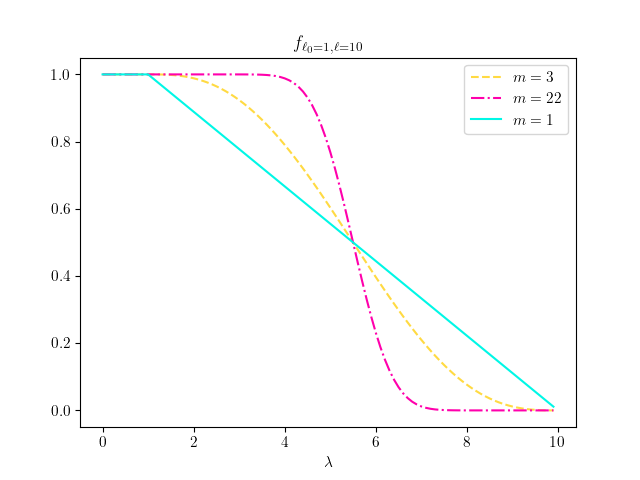
\includegraphics[width=1.1\linewidth]{Immagini/beta-functions.png}
	  \captionof{figure}{graphs of different functions in \(\mathcal{A}_{\beta}\) with \(\ell_0 = 1\), \(\ell = 10\) and \(3\) different values for \(m\). The incomplete beta function for \(m = 1\) coincides with the straight line, and becomes smoother and smoother with increasing \(m\).}
	  \label{fig:beta-functions}
	\end{minipage}
	\begin{minipage}{.45\textwidth}
	  \centering
	  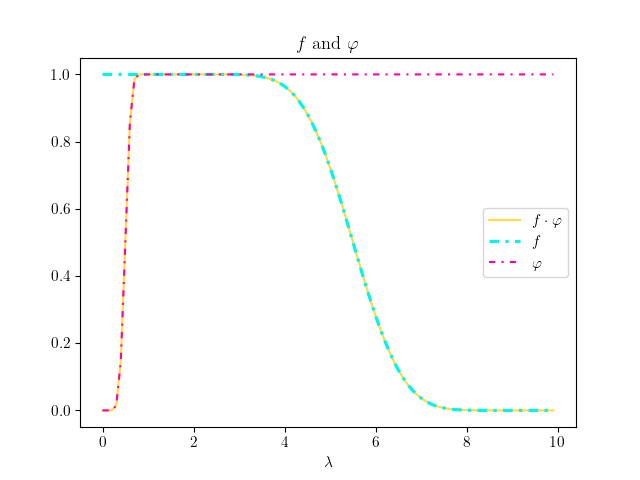
\includegraphics[width=1.1\linewidth]{Immagini/beta-functions-proof-bound.png}
	  \captionof{figure}{graphs of \(f\) and \(\varphi\) with \(\ell_0 = 1\), \(\ell=10\) and \(m = 14\), used in lemma \ref{lemma:J-sobolev-condition} to place a bound on \(J\). By taking the product of the two functions we obtain one that starts and ends at \(0\), and so can be used to apply the Sobolev energy condition.}
	  \label{fig:beta-functions-proof-bound}
	\end{minipage}
	\end{figure}

Now, assuming an additional condition on the stress energy tensor (or equivalently on the Ricci tensor), we are able to prove the following

\begin{lemma}
	\label{lemma:J-sobolev-condition}
	Assume the Sobolev condition holds, and the quantity \(\rho(\lambda) \coloneqq R_{\mu\nu}U^{\mu}U^{\nu}(\lambda) \) is lower controlled by \(\rho_0\) in \([0, \ell_0] \subseteq [0, \ell]\), or in other words
	\[
	   R_{\mu\nu}U^{\mu}U^{\nu}(\lambda) \ge \rho_0 \quad\quad \forall\lambda\in [0, \ell_0].
   \]
	Then for any \(f\in \mathcal{A}_{\beta}\) it holds:
	\begin{equation}
		\label{eq:J-sobolev-condition}
		J[f] \le (n - 2)\mathcal{V}_{\beta} \coloneqq -(1-A_m)\rho_0\ell_0 + \frac{Q_mC_m}{\ell_0^{2m-1}} + Q_0A_m\ell + \frac{(n - 2)B_m}{\ell - \ell_0} + \frac{Q_mC_m}{(\ell-\ell_0)^{2m-1}}.
	\end{equation}
\end{lemma}

\begin{proof}
	The proof of this lemma can be found in \cite{fewster2020new} as lemma \(4.1\), and it proceeds as follows. Define a piecewise smooth function \(\varphi\) on \([0,\ell]\) by:
	\[
	\varphi(\lambda) = 
	\begin{cases}
		I(m, m;\frac{\lambda}{\ell_0}) \quad \hfill \lambda \in [0, \ell_0) \\
		1 \hfill \lambda \in [\ell_0, \ell]
	\end{cases}	
	\]
	
	It's possible to see that \(\varphi f \in W_0^m([0,\ell])\), so writing \(f^2 = (\varphi f)^2 + (1 - \varphi^2)\) we have:
	\begin{align*}
		\int_0^{\ell} f(\lambda)^2\rho(\lambda) &\ge \int_0^{\ell} (1 - \varphi(\lambda)^2)\rho(\lambda)d\lambda - Q_m(\gamma) \vert\vert (\varphi f)^{(m)}\vert\vert^2 - Q_0(\gamma) \vert\vert \varphi f\vert\vert^2 \\
		&\ge  \rho_0\int_0^{\ell} (1 - \varphi(\lambda)^2)d\lambda - Q_m(\gamma) \vert\vert (\varphi f)^{(m)}\vert\vert^2 - Q_0(\gamma) \vert\vert \varphi f\vert\vert^2.
	\end{align*}

	Moreover, the norms of the functions can be analytically computed for the specific choices that we made:
	\[
		\vert\vert \varphi f\vert\vert^2 = A_m\ell_0 + A_m(\ell - \ell_0)\quad
		\vert\vert (\varphi f)^{(m)}\vert\vert^2 = \frac{C_m}{\ell_0^{2m - 1}} + \frac{C_m}{(\ell - \ell_0)^{2m - 1}}
		\quad
		\vert\vert f'\vert\vert^2 = \frac{B_m}{\ell - \ell_0}
	\]
	Thus,
	\[
		J[f] \le \frac{(n - 2)B_m}{\ell - \ell_0} + \frac{Q_mC_m}{\ell_0^{2m - 1}} + \frac{Q_mC_m}{(\ell - \ell_0)^{2m - 1}} + Q_0A_m\ell - \rho_0\ell_0(1 - A_m) \coloneqq (n-2)\mathcal{V}_{\beta},
	\]
	and the estimate is complete.
\end{proof}

\begin{SCfigure}
	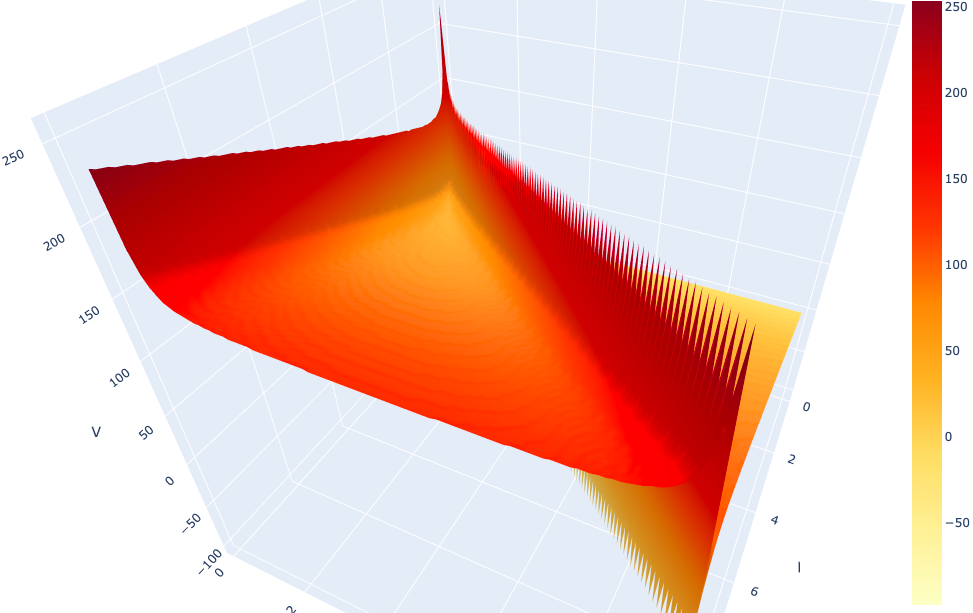
\includegraphics[scale=0.28]{Immagini/V-beta.png}
	\caption[]{plot of \(\mathcal{V}_{\beta}(\ell_0, \ell)\) (\(\hat{z}\) axis). On the right it appears part of the \(\ell\) axis, while the hidden one corresponds to \(\ell_0\). The color-scale should help to spot out the minimum of the visualized sheet.}
	\label{fig:V-beta}
\end{SCfigure}

Now that for each function \(f_{\ell_0, \ell} \in \mathcal{A}_{\beta}\) we have an estimate for \(J\left[f_{\ell_0, \ell}\right] \le (n-2)\mathcal{V}_{\beta}(\ell_0, \ell)\), we can finally pursue the variational strategy: we need to minimize \(\mathcal{V}_{\beta}(\ell_0, \ell)\) on \(\ell \ge \ell_0\). In order to do so we will first minimize along \(\ell\), keeping \(\ell_0\) fixed, and then proceed to a second minimization over this last parameter.

The first optimization has been already performed in \cite{fewster2020new}, even if in their computation they neglect some terms that instead will be relevant for us, because of the different regime of approximation that we will need to set. Let then us do that, with the additional restriction of \(m = 1\): in the following this request will always be fulfilled, so this is the most general we need to be, but this procedure could be generalized to arbitrary \(m\) at the price of solving a higher order algebraic equation.

\begin{prop}
    For \(m = 1\), the bound optimized on \(\ell \ge \ell_0\) is
    \[
      (n-2)\mathcal{V}_{\beta}(\ell_0) = (A_1 - 1)\rho_0\ell_0 + \frac{Q_1C_1}{\ell_0} + 2 \sqrt{(n - 2)A_1B_1Q_0}   
    \]
    and is obtained for:
    \[
    \tilde{\ell} = \ell_0\left(1 + \sqrt{\frac{(n - 2) B_1}{A_1 Q_0\ell_0^2}}\right)    
    \]
\end{prop}

\begin{proof}
    The proof is very similar to the one given in \cite{fewster2020new}, but we have to pay attention to keep all the terms relevant for us.
	\noindent
    Set \(\ell = \ell_0\left(1 + B_1\mu\right)\), so that the constraint \(\ell\ge\ell_0\) becomes simply \(\mu \ge 0\).
    % The interesting case presents when \(\mu \ge 1\), for which \(\frac{1}{\mu^{2m - 1}} \le \frac{1}{\mu} \) (in particular in subsection \ref{subsec:non-min-EKG-theory} we will focus on the \(m = 1\) case, where the equality holds). 
	The expression in \(\eqref{eq:J-sobolev-condition}\) reduces to:
    \begin{align*}
        \mathcal{V}(\ell, \ell_0) &= E + F\mu + \frac{G}{\mu} \\
        E &= (A_m - 1)\rho_0\ell_0 + Q_0A_m\ell_0 + \frac{Q_mC_m}{\ell_0}\\
        F &= Q_0A_mB_m\ell_0 \\
        G &= \frac{n- 2}{\ell_0} + \frac{Q_mC_m}{B_m\ell_0}
    \end{align*}
    Imposing the first derivative w.r.t \(\ell\) of \(\mathcal{V}_{\beta}\) to be zero, it is easy to obtain:
    \[
    \tilde{\mu} = \sqrt{\frac{G}{F}} =  \sqrt{\frac{n - 2}{A_1B_1Q_0\ell_0^2}}.
    \]
	where we neglected the second term of \(G\) under the assumption \(Q_1 \ll 1\); in the following we will see that \(Q_1 \sim \left(\frac{T}{T_{Pl}}\right)^2\), so assuming \(Q_1 \ll 1\) corresponds to be in the temperature regime where \(\left(\frac{T}{T_{Pl}}\right)^2 \ll 1\), which is not particularly restrictive as also the analysis of black hole evaporation is performed under the same assumption.
\end{proof}

Now we reduced to a bound that only depends on \(\ell_0\) (and some other global feature of the system, summarized within \(Q_0\) and \(Q_m\)); in light of the variational strategy, let us finally proceed to the last minimization and find the optimal value for \(\ell_0\)\footnote{Actually, there were several possibilities that could have been explored with the aim of providing an estimate for \(\ell_0\). The first idea was to pick some constant \(\ell_0\) (which is what has been done in \cite{fewster2020new}), fixed to be some relevant physical quantity, but we haven't been able to formulate one particularly convincing. Besides, requiring \(\ell_0\) to be constant in a background that will be dynamic didn't seem particularly reasonable after all, so we decided to minimize \(\mathcal{V}_{\beta}\) - and finally outlined the variational procedure.}. 

\begin{prop}
	Assuming \(\rho_0 < 0\) the optimal bound, minimized along \(\ell_0\), is:

	\begin{equation}
		\label{eq:minimized-V-beta}
		\mathcal{V}_{\beta} = \frac{5}{6}\sqrt{\frac{3}{2}Q_1 \vert\rho_0\vert} + 2 \sqrt{(n - 2)A_1B_1Q_0}
	\end{equation}

	corresponding to \(\tilde{\ell}_0^2 = - \frac{3Q_1}{2\rho_0}\)
\end{prop}
\begin{proof}
	The computation is very similar to the preceding one, as in particular the shape of the function to be minimized is exactly the same.
\end{proof}

Lemma \ref{lemma:generalized-area-theorem} can now immediately tell us that, in an asymptotically flat spacetime, wherever on the null generators of the black horizon the Sobolev energy condition holds and \(R_{\mu\nu}U^{\mu}U^{\nu} \ge \rho_0\), then the instantaneous rate of expansion of the cross-sectional area is constrained by
\begin{equation}
	\label{eq:area-sobolev-condition}
	U_{\mu}\mathrm{H}^{\mu} \ge - \mathcal{V}_{\beta} \implies \delta_U\mathcal{A}_{\mathscr{H}_1} = \int_{\mathscr{H}_1} \mathrm{H}^{\mu}(p)U_{\mu} \ge - \mathcal{V}_{\beta}\cdot\mathcal{A}_{\mathscr{H}_1},
\end{equation}
where, again, the implication is possible thanks to lemma \ref{lemma:variation-area}. We will argue later that the assumption \(\rho(\lambda) \ge \rho_0\) in a small interval of the affine parameter is well motivated, and we will find \(\rho_0 < 0\), so \eqref{eq:minimized-V-beta} is well defined, and \(\mathcal{V}_{\beta} >0\). This means we have proved that the rate of change of the area of the horizon near the reference ``time instance'' given by \(\Sigma_1\) cannot be lower than a certain - negative - rate!

Equation \eqref{eq:area-sobolev-condition} can then truly claim to be a first non trivial generalization of Hawking's area theorem: it is still placing a lower bound on the rate of evolution of the area, but, as the bound is negative this time, it can - in principle - resolve the tension with the quantum phenomenon of evaporation, now potentially allowed.
	
Notice however that, conversely to the original theorem, we have only constrained the \emph{instantaneous} rate of change. Here it is not possible to directly set bounds on the average rate of evolution between \(2\) arbitrarily far Cauchy surfaces \(\Sigma_1\) and \(\Sigma_2\), as for that we would need to assume the Sobolev condition and the pointwise restriction \(\rho \ge \rho_0\) in the all region in between \(\Sigma_1\) and \(\Sigma_2\), which would mean a significant weakening of our result.

\subsection{The second idea -- a differential equation}
\label{subsec:E-L-optimization}
A potential weakness of the variational method is that, if the set \(\mathcal{A}\) onto which the optimization is performed is not chosen with enough care, its extremum may still lay very far from \(\inf J\). Referring to the above subsection \ref{subsec:V-optimization}, it might happen that even if \(\mathcal{V}_{\beta} > 0\), the actual \(\inf_{f\in C^{\infty}_{1,0}[0, \ell], \ell \ge 0}J\) is negative, and hence evaporation is not allowed.

Such question can only be completely resolved by finding the true infimum, or a set \(\mathcal{A}\) where the minimum is negative. We are not able to do that unfortunately, but we can look at our results and see if anything stands out. 

It may attract our attention the curious feature that the minimum of \(\mathcal{V}_{\beta}\) lays at finite \(\ell\): a simple heuristic argument instead suggests that a priori we should expect it to be at \(\ell \rightarrow +\infty\).

\(\ell\) is nothing but the maximum length of the support of the function \(f\). Ideally, in order to minimize \(J[f]\), we should expect \(f\) to be non zero wherever \(R_{\mu\nu}U^{\mu}U^{\nu}\) is positive, and null (or almost null) wherever \(R_{\mu\nu}U^{\mu}U^{\nu} < 0\). By cutting out the possibility of exploring for \(\lambda \ge \ell\) we might just miss out some regions where \(\rho(\lambda)\) is positive again. 

\noindent
Analogously, when energy conditions of the form above mentioned come into force, instead of optimizing \(J\) we try to minimize \(\vert\vert \nabla_U f\vert\vert^2 + B[f]\), and again - as \(f\) is required to go from \(1\) at \(\lambda = 0\) to \(0\) at \(\lambda = \ell\) - by pushing \(\ell\) as far away as possible we would suppress the norms of all the derivative of \(f\).

We may then wonder how reasonable is the result we have obtained in \eqref{eq:area-sobolev-condition}; to test it we developed an alternative method, that is a combination of an Euler-Lagrange approach and the variational method. Suppose again to start from an energy condition of the form
	\[
		\int_0^{\ell} f^2 R_{\mu\nu}U^{\mu}U^{\nu} \ge -B[f] \implies J[f] \le \vert\vert \nabla_U f\vert\vert^2 + B[f]
	\]
and then, instead of choosing any set \(\mathcal{A}\), we write an Euler-Lagrange equation - that doesn't depend on the metric - to minimize 
	\[
	\vert\vert \nabla_U f\vert\vert^2 + B[f] \quad\text{ with }\quad f(0) = 1 \quad \quad f(\ell) = 0.	
	\]

Even if this is the main idea, we can only apply the Sobolev energy condition to functions that have Dirichlet boundary conditions; with some work it is possible to get to a differential equation also in the general case, but one that is too hard to be solved - at least for us.
By reducing to the set of functions (here's why we say that this method is partially a variational estimation again)
\[
\mathcal{A}_{E.L.} \coloneqq \{f \quad \vert \quad \exists \ell_0 > 0 \text{ s.t. } f(\lambda \le \ell_0) \equiv 1\} \supset \mathcal{A}_{\beta}
\]
the problem becomes doable, and we obtain:
\begin{equation}
	\label{eq:V-euler-lagrange}
	\mathcal{V}_{E.L.}(\ell_0, \ell) = \sqrt{Q_0(n - 2 + Q_1)}\coth\left[\Omega_1(\ell- \ell_0)\right] + \sqrt{Q_0Q_1}\coth\left[\Omega_2\ell_0\right] + \vert \rho_0\vert\ell_0
\end{equation}
where
\[
\Omega_1^2 = \frac{Q_0}{n - 2 + Q_1} \quad \quad  \Omega_2^2 = \frac{Q_0}{Q_1}.
\]

All the main ideas behind this procedure have already been explained with enough detail in the present section or in \ref{subsec:V-optimization}, so we defer the computation that proves equation \eqref{eq:V-euler-lagrange} to appendix \ref{app:V-E-L-optimization}.

\begin{SCfigure}
	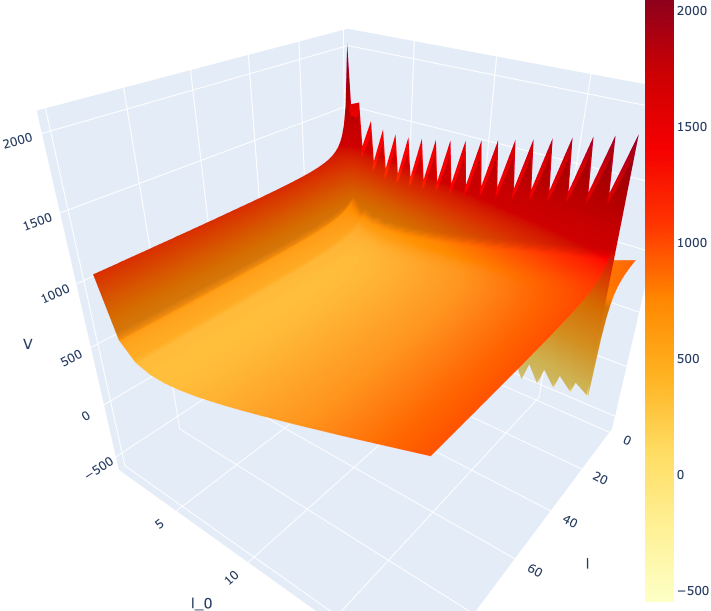
\includegraphics[scale=0.3]{Immagini/V-E-L.png}
	\caption[]{Plot of \(\mathcal{V}_{E.L.}(\ell_0, \ell)\); this plot can be directly compared to the one in figure \ref{fig:V-beta} and again it stands out that this time the minimum will lay at large \(\ell\).}
	\label{fig:V-E-L}
\end{SCfigure}

Once more, we minimize \(\mathcal{V}_{E.L.}(\ell_0, \ell)\) on \(\ell \ge \ell_0\) in order to recover the best possible bound on \(\inf J\). We immediately see that this time the minimum is found for \(\ell \rightarrow +\infty\): the only \(\ell-\)dependence is in \(\coth\left[\Omega_1(\ell- \ell_0)\right]\), which is monotonically descending towards \(1^+\).

For \(\ell_0\) instead, the minimum is found at \(\tilde{\ell}_0 = \sqrt{\frac{Q_1}{Q_0}}\sinh^{-1}\left(\sqrt{\frac{Q_0}{\vert\rho_0\vert}}\right)\), so that in the end we have
{\small
\begin{equation}
	\label{eq:minimized-V-E-L}
	U_{\mu}\mathrm{H}^{\mu} \ge - \frac{1}{n - 2}\mathcal{V}_{E.L.} =  \frac{1}{n - 2} \left\{ \sqrt{Q_0(n - 2 + Q_1)} + \sqrt{Q_1(Q_0 + \vert\rho_0\vert)} + \frac{3}{2}\sqrt{Q_1\vert\rho_0\vert} \right\}.
\end{equation}}

Notice that, even if \(\mathcal{A}_{E.L.}\) is a much larger set than \(\mathcal{A}_{\beta}\), the result in \eqref{eq:minimized-V-E-L} is very similar to the one in \eqref{eq:minimized-V-beta}; indeed only some coefficients are changed, but the qualitative behaviour is always the same, and in particular \(\mathcal{A}_{E.L.}\) stays negative.

\section{Comparison with the evaporation rate}
\label{sec:physical-interpretation-V}

Coherently, with the weakening of the energy condition we have obtained a weaker constraint: but what is the real physical impact of the new hypothesis we have taken?

As extensively argued above, \(\mathcal{V}\) represents the bound on the instantaneous rate of change of the area of the black hole horizon. In order to understand how reasonable it is the expression we have obtained, we would need to compare it to some relevant physical quantity; in this scenario we are lucky enough to have a particular appealing one: the rate of black hole evaporation.

With that in mind, we need to translate the mathematical expression of \(\mathcal{V}\) given in \(\eqref{eq:minimized-V-E-L}\) into a function of physical quantities only; once again we will let us be inspired by the work in section \(5.2\) of \cite{fewster2020new}, where Fewster and Kontou computed their bound in the specific framework of a non-minimally coupled classical Einstein-Klein Gordon theory.

They needed such a computation to test the hypothesis of some weakened singularity theorems within astrophysical scenarios; here instead we would like to analyze the evaporation of black holes, hence we will need a different regime of approximations.

\subsection{The non-minimally coupled Einstein Klein Gordon Theory}
\label{subsec:non-min-EKG-theory}
First of all let's try to compute some reasonable physical estimates of the coefficient \(Q_0\) and \(Q_m\). In order to do so we need to pick a specific field theory, and we will adopt a semiclassical gravity point of view, so quantum fields within a classical background geometry, where backreaction corrections are assumed small - and thus neglected.

Our choice happens to land on non-minimally coupled scalar fields: this is the typical classical field theory violating NEC, and thus the original black hole area theorem doesn't apply. They are scalar fields described by the Lagrangian density
\[
\mathcal{L}[\phi] = -\frac{1}{2}\left[\nabla_{\mu}\phi\nabla^{\mu}\phi   - (m^2 - \xi R)\phi^2\right]
\]
The corresponding stress-energy tensor is:
\begin{equation}
    T_{\mu\nu} = \nabla_{\mu}\phi\nabla_{\nu}\phi - \frac{1}{2}g_{\mu\nu}\left[\nabla_{\rho}\phi\nabla^{\rho}\phi - m^2\phi^2\right] + \xi\left(g_{\mu\nu}\square_g - \nabla_{\mu}\nabla_{\nu} + G_{\mu\nu}\right)\phi^2
\end{equation}
% La derivazione di https://alves-nickolas.github.io/pdf/Stress_Energy_Momentum_Tensor_for_a_Scalar_Field.pdf mi e' piaciuta
The conformal coupling is \(\xi_c = \frac{1}{4}\frac{n - 2}{n - 1}\), and we will only consider \(\xi\in [0,\xi_c]\);
now the following observation comes along.

\begin{prop}
    It is physically reasonable to impose that \(8\pi\xi\phi^2 < 1\).
\end{prop}

\begin{proof}
    The argument can be found in \cite{kontou2020energy} and starts by rearranging Einstein equations in the following form:
    \[
      \frac{1 - 8\pi\xi\phi^2}{8\pi}G_{\mu\nu} =  \underbrace{\nabla_{\mu}\phi\nabla_{\nu}\phi - \frac{1}{2}g_{\mu\nu}\left[\nabla_{\rho}\phi\nabla^{\rho}\phi - m^2\phi^2\right] - \xi\left(g_{\mu\nu}\square_g - \nabla_{\mu}\phi\nabla_{\nu}\right)\phi^2}_{T^{eff}_{\mu\nu}}.
    \]
    Notice that - for \(\xi > 0\) - the coefficient in front of \(G_{\mu\nu}\) vanishes for \(8\pi\xi\phi^2 = 1\); for such values of the field \(\phi\) the order of Einstein equations reduces, and so the initial value problem becomes ill-defined.

    When \(8\pi\xi\phi^2 \neq 1\) instead, Einstein equations become:

    \[
        G_{\mu\nu} = \frac{8\pi}{1 - 8\pi\xi\phi^2}T^{eff}_{\mu\nu},
    \]
    and so we can see that for \(8\pi\xi\phi^2 > 1\) we would have a negative ``effective Newton's constant''. 

    This is not a definitive proof that non-minimally coupled fields cannot access such high values (called \emph{trans-Planckian}), but it is more a motivation about why it seems reasonable to assume that bound. 
\end{proof}

From here onward we will assume that non-minimally coupled scalar fields will always obey the bound:
\[
\phi^2 < \frac{1}{8\pi\xi}.    
\]
Moreover we shall only consider \emph{massless} scalar fields; given that, it was shown in \cite{fewster2011singularity} and \cite{brown2018singularity} that the Ricci tensor contraction is bounded by a Sobolev-like energy condition.

\begin{prop}
    In the context of a massless non-minimally coupled Einstein-Klein Gordon field theory, the integral of the contraction of the Ricci tensor along any causal geodesic, weighted with any compactly supported real valued \(-\frac{1}{2}\)-density \(f\), is bounded by:

    \begin{equation}
        \int_{\gamma}f^2 R_{\mu\nu}U^{\mu}U^{\nu} \ge -Q\left(\vert\vert\nabla_U f \vert\vert^2 + \tilde{Q}^2 \vert\vert f\vert\vert^2\right).
    \end{equation}
    where 
    \[
    Q = \frac{32\pi\xi\phi_{max^2}}{1 - 8\pi\xi\phi_{max}
    ^2}
    \quad\quad
    \tilde{Q} = \frac{8\pi\xi\phi_{max}}{1 - 8\pi\xi\phi_{max}
    ^2}\sup_{\gamma}\vert \nabla_U\phi\vert.
    \]
\end{prop}

The proof of is lengthy and not particularly interesting for the scope of this thesis, so we defer it to appendix \ref{app:proof-EKG-bound}.

We have indeed found an energy condition of the form \(\eqref{eq:Sobolev-condition}\) with 
\[
m = 1 \quad\quad Q_0 = Q\cdot\tilde{Q}^2 \quad\quad Q_1 = Q 
\]

\subsection{The Kubo-Martin-Schwinger state}

In order to finally convert \(Q_0\) and \(Q_1\), we need to compute \(\phi_{max}\) and \(\sup_{\gamma}\vert \nabla_U\phi\vert\) in terms of some physical quantities; in principle the field values may be not bounded, but here we only aim at estimating what a reasonable value for \(\mathcal{V}\) would be.
Physically, it makes sense that the value of \(\phi_{max}\) is connected to some sort of background temperature, and we expect the higher \(T\) is, the higher values \(\phi\) might reach.

In order to establish this connection we now change setting, and consider a \emph{quantum} field theory with a minimally coupled massless scalar field in a Minkowski background metric; we aim at computing the Wick square of our field averaged in a thermal state of temperature \(T\). As choice of thermal state, we pick the Kubo-Martin-Schwinger (KMS) state with temperature \(T\), as in section \(5.2\) of \cite{fewster2020new}, where we can compute the desired quantity in a way analogous to what has been done in the final appendix of \cite{brown2018singularity}.

\begin{definition}
    The KMS state is defined as \dots
    %todo: studiare
\end{definition}

\begin{remark}
	The KMS state is a \emph{thermal equilibrium} state. This means we must be working with quasi-static black holes, which are evaporating so slowly that can be thought always in nearly thermal equilibrium with the background. This approximation should be well verified because, once again, it coincides with the temperature regime \(\frac{T}{T_{Pl}}\ll 1\).
\end{remark}

\begin{prop}
	\label{prop:wick-squares-KMS}
    The Wick square of the massless field, in a KMS thermal state of temperature \(T\), within a \(n\)-dimensional Minkowski spacetime, is given by:
    \begin{align*}
         \langle \colon \phi^2 \colon\rangle_T &= \frac{T^{n - 2}}{2^{n - 2}\pi^{\frac{n - 1}{2}}}\frac{\Gamma(n - 2)}{\Gamma\left(\frac{n - 1}{2}\right)}\zeta(n - 2) \\
        \langle \colon (\nabla_U\phi)^2 \colon\rangle_T &= \frac{nT^n}{2^{n - 1}\pi^{\frac{n - 1}{2}}} \frac{\Gamma(n)}{\Gamma\left(\frac{n + 1}{2}\right)} \zeta(n)
    \end{align*}

\end{prop}
    
\begin{proof}
    Given \(\beta = \frac{1}{k_BT}\) the \(2\)-point function of the state is:
	\[
	W^{(2)}_T(x, x') = \int \frac{d^{n - 1}\mathbf{k}}{(2\pi)^{n - 1}}\frac{1}{2k^0(\mathbf{k})} \left(\frac{e^{-ik^{\mu}(x_{\mu} - x'_{\mu})}}{1 - e^{-\beta k^0(\mathbf{k})}} + \frac{e^{ik^{\mu}(x_{\mu} - x'_{\mu})}}{e^{\beta k^0(\mathbf{k})} - 1}\right). 
	\]

	As we are dealing with a massless scalar field, the dispersion relation is \(k^0(\mathbf{k}) = \vert \mathbf{k}\vert\) (the field is on-shell).

	For the ground state \(2\)-point function we need to take the limit \(T\rightarrow 0\), or \(\beta\rightarrow +\infty\), and obtain
	\[
	W^{(2)}_0(x, x') = \int \frac{d^{n - 1}\mathbf{k}}{(2\pi)^{n - 1}}\frac{1}{2k^0(\mathbf{k})} e^{-ik^{\mu}(x_{\mu} - x'_{\mu})}. 
	\]
	The Wick square is defined to be:
	\[
		\langle \colon \phi^2 \colon\rangle_T = \lim_{x'\rightarrow x} \left[W^{(2)}_T(x, x') - W^{(2)}_0(x, x')\right]
	\]
	The above expression can be simply worked out to be:
	\begin{align*}
		\langle \colon \phi^2 \colon\rangle_T &= \underbrace{\frac{2\pi^{\frac{n-1}{2}}}{\Gamma(\frac{n - 1}{2})}}_{\Omega_{n - 2}}\frac{1}{(2\pi)^{n - 1}}\frac{1}{\beta^{n - 2}}\int_0^{+\infty}dx \frac{x^{n - 3}}{e^x - 1} =\\
		&= \frac{T^{n - 2}}{2^{n - 2}\pi^{\frac{n - 1}{2}}}\frac{\Gamma(n - 2)}{\Gamma\left(\frac{n - 1}{2}\right)}\zeta(n - 2)
	\end{align*}
	The second inequality can be worked out in a similar way, being careful that this time there is an angular dependance because of the additional factor \((k_{\mu}U^{\mu})^2\), originated by the \(U\)-derivatives. This factor adds a \(k^2\) power to the radial part of the integral, and an angular factor:
	\[
	\int_0^{\pi} \sin\theta^{n - 3} (1 - \cos\theta)^2 d\theta = \frac{n\sqrt{\pi}}{2}\frac{\Gamma\left(\frac{n - 2}{2}\right)}{\Gamma\left(\frac{n + 1}{2}\right)}.
	\]
	So the final result becomes:
	\begin{align*}
		\langle \colon (\nabla_U\phi)^2 \colon\rangle_T &= 
		\underbrace{\frac{2\pi^{\frac{n-2}{2}}}{\Gamma(\frac{n - 2}{2})}}_{\Omega_{n - 3}} \cdot \frac{n\sqrt{\pi}}{2}\frac{\Gamma\left(\frac{n - 2}{2}\right)}{\Gamma\left(\frac{n + 1}{2}\right)} \cdot \frac{1}{(2\pi)^{n - 1}}\frac{1}{\beta^{n}}\int_0^{+\infty}dx \frac{x^{n - 1}}{e^x - 1} = \\
		&= \frac{nT^n}{2^{n - 1}\pi^{\frac{n - 1}{2}}} \frac{\Gamma(n)}{\Gamma\left(\frac{n + 1}{2}\right)} \zeta(n).
	\end{align*}
\end{proof}

At last we estimate the maximum values of the \emph{classical} E-KG field and its derivative by the ansatz 
\begin{align*}
	\phi_{\max}^2 &\simeq \langle \colon \phi^2 \colon\rangle_T,\\
	\sup_{\gamma}\vert \nabla_U\phi\vert &\simeq \langle \colon (\nabla_U\phi)^2 \colon\rangle_T.
\end{align*}
Restoring units and reducing to \(n = 4\) spacetime dimensions, we eventually obtain:
\begin{align}
	\label{eq:KMS_Q_1}
    Q_1 &= \underbrace{\frac{16\pi\xi}{3}}_{\alpha} \left(\frac{T}{T_{Pl}}\right)^2,\\
    Q_0 &= \underbrace{\frac{32\pi^6\xi^3}{405}}_{\gamma}\left(\frac{k_B}{\hbar}\right)^2 \frac{T^8}{T_{Pl}^6}.
\end{align}

Again, this is of course not a rigorous computation of the coefficients, but it's a meaningful approximation pursued in an instructive toy-model, that can give us some encouraging insights on the underlying complicated physics.

For the purpose of the following analysis we will identify \(T\) with the Hawking temperature of the black hole \(\eqref{eq:hawking-temperature}\):
\[
T_H = \frac{\hbar c^3}{8\pi Gk_B}\frac{1}{M}    
\]
    
\begin{remark}
	The toy model we relied on in this section has, of course, many limitations. One we have tried to resolve is due to the definition of the \(2\)-point function of KMS states - used to prove proposition \ref{prop:wick-squares-KMS} - only in Minkowski spacetime. The proper state to describe a black hole in thermal equilibrium within an underlying Schwarzschild geometry is the Hartle-Hawking state \cite[]{hartle1993path}. This state has been proved to be equivalent to the double KMS state with temperature equal to Hawking temperature, first in \cite[]{jacobson1994note, sanders2015construction} (with the path integral formulation), and lately in \cite[]{higuchi2022hartle} by means of the Schwinger-Keldysh operator formalism. Unfortunately the \(2\) point function is a little more complicated than the one in the flat space case:
	\[
	W_{HH}(x, x') = \int_{0}^{+\infty} \frac{d\omega}{2\omega} \sum_{\sigma}\phi_{\omega\sigma}(x)\phi_{\omega\sigma}(x')\left(\frac{e^{-i\omega(t - t')}}{1 - e^{-\beta \omega}} + \frac{e^{i\omega(t - t')}}{e^{\beta \omega} - 1}\right),
	\]
	where \(\{\phi_{\omega\sigma}(x)\}\) are a basis of the set solutions to the equations of motion. In flat spacetime the factor \(\sum_{\sigma}\phi_{\omega\sigma}(x)\phi_{\omega\sigma}(x')\) simply reduces to 
	\[
		\int_{\vert k \vert = \omega}	\frac{dk^{n - 1}}{(2\pi)^{n - 1}} e^{-i\vec{k}\cdot \vec{x}},
	\]
	but as for now we didn't manage to work it out in the Schwarzschild case. Working out the additional temperature dependence - if any - given by such factor would be enough to properly generalize our method to Schwarzschild.
\end{remark}

\subsection{Limited violations}
\label{subsec:rho-0-estimation}

In order to estimate the value of the functional \(J[f]\) we required 
\[
	\rho (\lambda)\coloneqq R_{\mu\nu}U^{\mu}U^{\nu}\ge -\vert\rho_0\vert
\] 
for \(\lambda\in [0, \ell_0]\); this is again a pointwise requirement, but notice that, as the lower bound is negative, it is not ruled out by the argument in \ref{th:quantum-violation-pointwise-conditions}.

It has been for long debated whether such contractions of the stress energy tensor should be finite or not; in literature there can be found arguments for both sides, and indeed a lot of attention must be payed to what contraction exactly is going to be computed. The presence of a coordinate singularity, and the lack of an analytical expression for the \(4\)-dimensional stress-tensor in the Unruh or Hartle-Hawking state complicate the matter, but we will try to argue that - as the one on the horizon is \emph{just} a coordinate singularity - the contraction of \(T_{\mu\nu}\) with the tangent field of the null generators shall be always finite.

Let us again work within the framework of non-minimally coupled scalar fields, with \(\xi\in[0,\xi_c]\); developing a general treatment is very difficult because of the features mentioned above, but at the two extremities of this interval  a few observation can be inferred.

For \(\xi = 0\) the field becomes minimally coupled; the classical minimally coupled Klein-Gordon field actually obeys the Null Energy condition, but this doesn't mean that the quantized field shouldn't bear any surprise.
Indeed, in \cite{levi2016versatile} Levi and Ori have been able to overcome many of the complications for the computation of a renormalized stress tensor in the Unruh vacuum, and managed to run some numerical simulations to estimate \(\rho\) in the outer proximity of the horizon, within a background Schwarzschild metric. 
Recasted with our convention (for us their \(a\) needs to be \(1\)), their result is 
\begin{equation}
	\label{eq:rho-Levi-Ori}
	\rho \simeq -2.7\cdot 10^{-7} \frac{\hbar}{M^{4}} 
\end{equation}
(where \(M\) is the mass of the black hole). This supports the legitimacy of our additional assumption, at least for large enough black holes, and suggests that such a condition might be commonly satisfied even with a rather small value of \(\vert\rho_0\vert\). The most important features of Levi and Ori's result~\eqref{eq:rho-Levi-Ori} are the negative sign and the \(M^{-4}\) dependence: we will see this is ultimately determining the temperature dependence of our bound \(\mathcal{V}\), and hence any variation of this power law would have major impact on our conclusions.

The field we considered in~\ref{subsec:non-min-EKG-theory} however, is not minimally-coupled. Anyways, for conformally coupled fields a very similar result should hold. 
In~\cite{visser1997gravitational} Visser develops a semi-analytical computation for the renormalized stress energy tensor (RSET) of a massless scalar field conformally coupled to the background Schwarzschild metric, averaged on the Unruh vacuum state. At first glance it seems that he proves that such contractions cannot be bounded, and actually has a pole divergence on the black hole horizon; at a closer look however, it is possible to realize that none of the contractions computed in~\cite{visser1997gravitational} is the one we need, because of the particular coordinate system he works with. In fact, it is necessary to rewrite the components of the stress tensor derived by Visser within the Kruskal-Szekeres coordinate system, and in such system we really are able to derive \(R_{\mu\nu}U^{\mu}U^{\nu}\). The computation is not particularly difficult, but is somewhat long and thorny, and shouldn't distract us from the main discussion: we will carefully explain the model and derive the result in appendix~\ref{app:visser}. At last, we find again that \(\rho\) is bounded by a negative quantity, that scales with \(M^{-4}\)! Precisely, the result in \eqref{eq:contraction-stress-tensor} traduces to:
\[
	\rho \simeq \frac{9}{10(16\pi)^2} \cdot \frac{e}{V_0^2} \cdot \frac{\hbar}{(2M)^4}.
\] 
The advantage of a semi-analytical model is that it allows us to extrapolate how minimal are the requirements from which those two main features arise; in particular the same features should be valid also for all the fields with coupling \(\xi\) within the all interval \([0,\xi_c]\), even if we can't compute the exact coefficient because of our ignorance of the trace of the stress tensor in the general case.

\subsection{Comparison with the evaporation rate}
By substituting \(\rho_0\) into~\eqref{eq:minimized-V-beta} or~\eqref{eq:minimized-V-E-L} we finally get:
\begin{equation}
	\label{eq:KMS-minimized-V-beta}
	\mathcal{V}_{min} = 5\cdot10^{-3} \cdot (8\pi)^2\sqrt{\alpha} \frac{Gk_B^3}{\hbar^2} \cdot T^3 + \mathcal{O}\left(\left(\frac{T}{T_{Pl}}\right)^4\right),
\end{equation}

where \(\alpha \sim \frac{16\pi\xi}{3}\) is the dimensionless constant that relates \(Q_1\) to its temperature dependence, as computed in \(\eqref{eq:KMS_Q_1}\).

This result is extremely interesting: despite all the approximations and arguable ansatzs, we recovered the same temperature power law of the evaporation rate, computed by a totally different method! 

\begin{remark}
	Notice that a priori it was not at all clear that we would have found a \(T^3\) dependence: when \(Q_1\) is connected to the temperature - as for dimensional argument \(\left[Q_1\right] = 0\) - we know there must be a combination of constants with the dimension of a temperature (which happens to be the Planck temperature), so, in principle, there could have been factors \(\left(\frac{T}{T_{Pl}}\right)^a\) in \(\tilde{\ell}_0\) that would have changed the power law.
\end{remark}

In particular, a direct comparison with the formula in \(\eqref{eq:evaporation-rate}\) - recalling that  \(\beta \sim \mathcal{O}(10^{-5})\) - tells us that \(\mathcal{V}_{min}\) is allowing that rate of evaporation for 
\[
\alpha \gtrsim \frac{1}{400} \iff \xi \gtrsim 1.49 \times 10^{-4}	
\]
so in principle the field might be very weakly coupled (for the comparison we used the value of \(\rho_0\) as computed by Levi and Ori in~\cite[]{levi2016versatile}). This coefficient comparison is way less meaningful though, as they are very model dependent, and therefore it is not clear how reflective of the underlying physics they are.

Finally, it should also be noticed how the pointwise restriction on \(\rho\) cannot be simply get rid of. The key point is that the test function of the variational method needs to start from \(1\) at \(\lambda = 0\), while the averaged conditions can only use functions with Dirichlet boundary conditions. It looks very interesting then the fact that such term gives one of the most relevant contributions to \(\mathcal{V}\), and indeed how the trace anomaly seems to be intimately connected to Hawking radiation. 

The question we would like to ask ourselves now is: how robust is this result, and in particular the \(T^3\) dependence? Is it just an artifact of the specific examples and approximations we have been using, or is it the signal of a more general behaviour? 

\section{The Smeared Null Energy Condition}
The Smeared Null Energy condition is a bound on a contraction of the stress energy tensor, and it has been been first proposed in~\cite{freivogel2018smeared}; it is of particular interest to us because a Penrose-like singularity theorem has been proved from it~\cite{freivogel2020return} and because all the work done in section~\ref{sec:physical-interpretation-V} is nearly directly applicable, as SNEC belongs to the class of Sobolev energy conditions.

\begin{definition}
	The Smeared Null Energy Condition asks that, on any achronal portion of a null geodesic it holds:
	\begin{equation}
		\label{eq:SNEC}
		\forall f \in C_0^2[(-\infty, +\infty)] \quad\quad \int f^2(\lambda)\langle T_{\mu\nu}U^{\mu}U^{\nu}(\lambda) \rangle d\lambda \ge -\frac{4B}{G_N}\vert\vert \nabla_U f\vert\vert^2
	\end{equation}
\end{definition}

It stands out immediately that \(\eqref{eq:SNEC}\) is of the form of \(\eqref{eq:Sobolev-condition}\), with 
\[
m = 1 \quad \quad Q_0 = 0 \quad \quad Q_1 = 4B.	
\]
But, there is a ``but''. Here \(B\), and hence \(Q_1\) is asked to be a \emph{state independent} constant, namely it can only depend on the field theory we choose to populate our universe, but not the state we average the stress tensor in. 
Indeed we will see shortly that this requirement will have some dramatic consequences on the connection of \(\mathcal{V}\) to temperature.

\subsection{Variational estimation}
It is immediate to re-apply the analysis of sections \ref{subsec:variational-estimation} and \ref{subsec:E-L-optimization} to this specific energy condition.

In particular we can set \(Q_0 = 0\) in \eqref{eq:minimized-V-E-L} to obtain
\[
	\mathcal{V}_{SNEC} = \frac{5}{4}\sqrt{Q_1\vert\rho_0\vert};
\]
However, this time \(Q_1 = \frac{4B}{G_N}\) is state independent, so adopting the same estimation for \(\rho_0\) as justified in~\ref{subsec:rho-0-estimation}:
\[
\mathcal{V}_{SNEC} \simeq (13\cdot 10^{- 4})\sqrt{B} \cdot \sqrt{\frac{G}{\hbar^3}}k_B^2T^2.	
\] 

We have found again that black hole evaporation is allowed, but the bound depends on \(T\) with a quadratic power law; this means that the evaporation rate lies in the allowed region for \(T \le \tilde{T}\), where
\[
\frac{\tilde{T}}{T_{Pl}} = \frac{104\pi}{\beta}\cdot 10^{-4}\sqrt{B} \simeq 3\sqrt{B} \cdot 10^3.
\]
SNEC was proven in \cite{leichenauer2019upper} in the context of gravity induced on a brane, and in that specific case \(B\) was fixed to the value of \(\frac{1}{32\pi}\). However, as remarked in \ref{sec:SNEC}, it is often reasonable to consider \(B\ll 1\), condition that potentially could reduce dramatically the regime of validity of the bound we have found. This is consistent with the interpretation we have given of \(B\): \(B \ll 1\) would mean that, for the chosen field theory, semiclassical gravity is well under control, and therefore black holes can only evaporate ``very slowly''. 
\noindent
In other words, we expect rate of evaporation computed in \(\eqref{eq:evaporation-rate}\) to be allowed throughout the all region \(T\le T_{Pl}\) only with a field theory that induces proper non-classical effects (as large ``enough'' violations of \(T_{\mu\nu}U^{\mu}U^{\nu}\) for example), in which case \(B\) will be at least of order \(10^{-6}\) and \(\tilde{T} \gtrsim T_{Pl}\).

Finally, if we were to believe SNEC to hold also with values of \(B\) small enough for having \(\tilde{T} < T_{Pl}\), we might expect that at \(\tilde{T}\), other terms of \(\mathcal{V}\) become relevant, and push the bound above the rate of evaporation again.
A possible attempt to find such terms would be to modify SNEC so to include terms depending on the curvature, as it has been attempted in \cite{kontou2015quantum}.
% \VS{Cerca di aggiungere termini di curvatura!}

\section{State independent bounds}
\label{subsec:state-independent-bounds}
It is reasonable to expect, from a semi-classical energy condition at least, that at low Hawking temperatures only slow black hole evaporation is allowed; as \(T_H\) increases the evaporation is expected to get faster and faster, and eventually we might encounter a breakdown of the bound given by the semiclassical energy condition, possibly close to the Planck temperature, where in fact we expect any semi classical approximation to fail.
\noindent
The translation of this intuition onto our work is that we expect the bound on the evaporation rate \(R_{Ev} \le \mathcal{V}\), to pick up temperature corrections - again in a sort of perturbative framework - of at ``least'' degree \(3\).
In other words, if we are able to expand \(\mathcal{V}\) in terms of the Hawking temperature
\[
\mathcal{V} = v_0 + v_1T_H + v_2T_H^2 + v_3T_H^3 + \ldots	
\]
we expect at least one of the coefficients among \(\{v_0, v_1, v_2, v_3\}\) to be non-zero; if that wasn't the case in fact the evaporation rate in \(\eqref{eq:evaporation-rate}\) would be prohibited for some semi-classical regimes, but allowed when \(T_H\) is higher (see figures \ref{fig:state-independent-bounds} for a graphical representation).

This sets some restrictions onto the energy conditions we start from, in case they are state-independent. We are going to prove the following:
\begin{prop}
	State independent energy conditions in the form of a Sobolev condition with \(Q_0 = 0 \) must have \(m \le 2\) in order to be the same or lower order in temperature, compared to the predicted black hole evaporation rate.
\end{prop}
\begin{proof}
	The reason why we need to ask for state-independence is that this way we make sure we don't have any non trivial contribution of the temperature to the coefficients \(Q_0\) and \(Q_m\). If they were to depend on \(T\) in principle it is not easy to restrict what dependence they should bear, as the presence of \(T_{Pl}\) invalids the power of dimensional analysis.

	Again, it is enough to look at the set \(\mathcal{V}_{\beta}\) of incomplete beta functions, and study the bound retrieved in lemma \ref{lemma:J-sobolev-condition}:
	\[
	(n - 2)\mathcal{V}_{\beta}(\ell, \ell_0) \coloneqq \frac{(n - 2) B_m}{\ell - \ell_0} + \frac{Q_mC_m}{\ell_0^{2m - 1}} + \frac{Q_mC_m}{(\ell - \ell_0)^{2m - 1}}	+ Q_0A_m\ell + \vert\rho_0\vert\ell_0(1 - A_m)
	\]
	As in subsection \ref{subsec:V-optimization} we set out to minimize \(\mathcal{V}\) with respect to \(\ell \ge \ell_0\). Again we choose to parameterize \(\ell = (1 + B_m\mu)\ell_0\); however, this time we need to deal with a \(2m\)-degree equation, which in general is not explicitly solvable.
	\[
		(n - 2)\frac{d\mathcal{V}}{d\mu} = -\frac{n - 2}{\ell_0} \frac{1}{\mu^2} + \frac{Q_mC_m}{(B_m \ell_0)^{2m - 1}} \cdot \frac{1 - 2m}{\mu^{2m}} + Q_0A_mB_m\ell_0 = 0.
	\]
	This is not a big deal though: for our goal we are only interested to the temperature dependence of the minimum point \(\tilde{\mu}\), and that can only come from the minimizing \(\ell_0\). The equation we have to solve is of the form:
	\[
	\alpha \ell_0 \mu^{2m} - \frac{\beta}{\ell_0}\mu^{2m - 2} - \frac{\gamma}{\ell_0^{2m - 1}} = 0,
	\]
	so, for the equation to be homogeneous in \(\ell_0\) it must be\footnote{explicitly, multiplying by \(\ell_0^{2m - 1}\) the equation becomes \(\alpha(\mu\ell_0)^{2m} - \beta(\mu\ell_0)^{2m -2} - \gamma = 0\)}:
	\[
	\tilde{\mu} \propto \frac{1}{\ell_0}.
	\]
	Plugging back \(\mu = \frac{L}{\ell_0}\) into \(\mathcal{V}\) we obtain:
	\[
		(n - 2)\mathcal{V}_{\beta}(\ell_0) = \underbrace{\frac{(n - 2)}{L} + \frac{Q_mC_m}{L^{2m - 1}} + Q_0A_mB_mL}_{\text{constant}} + \frac{Q_mC_m}{\ell_0^{2m - 1}} + Q_0A_m\ell_0 + \vert\rho_0\vert\ell_0(1 - A_m)	
	\]
	and minimizing along \(\ell_0\) we have:
	\begin{equation}
		\label{eq:state-indipendent-minimal-l0}
		\tilde{\ell}_0	= \left(\frac{Q_0 A_m + \vert\rho_0\vert (1 - A_m)}{(2m - 1)Q_mC_m}\right)^{-\frac{1}{2m}}.
	\end{equation}
	In the limit where \(Q_0 \rightarrow 0\)
	\[
		\mathcal{V}_{\beta} \propto const + \vert \rho_0\vert^{1 - \frac{1}{2m}}.
	\]
	Here we think it makes sense to neglect the additional additive constant as it seems plausible that it only is an artifact of the ``small'' set of functions we are using for the minimization. This is for two reasons: there is no such constant in \eqref{eq:minimized-V-E-L} (where the minimization was indeed run on a larger set), and physically we should expect no evaporation at all when \(T_H = 0\).

	Finally, motivated once more by the work in \cite{levi2016versatile} and in appendix \ref{app:visser}, we take \(\rho_0 \propto T^4\), so that \(\mathcal{V} \propto T^{4 - \frac{2}{m}}\). 
	Hence, 
	\[
		4 - \frac{2}{m} \le 3 \iff m \le 2,	
	\]
	which is indeed the aim of the proof.
\end{proof}
As to have a gauge, from equation \eqref{eq:state-indipendent-minimal-l0} we can see that it is reasonable to approximate \(Q_0\simeq 0\) whenever \(Q_0 \ll \vert\rho_0(T_{min})\vert\). How to choose \(T_{min}\) depends on what scenario we are studying: for astrophysical black holes formed after gravitational collapse the initial mass is \(\sim 10 M_{\astrosun}\), corresponding \(T_H \simeq \SI{6}{\nano\kelvin}\); supermassive black holes instead have much larger masses, corresponding to even lower temperatures.

Unfortunately, when we cannot approximate \(Q_0 \simeq 0\) we are not able to infer anything as powerful, because the bound reduces to 
\begin{equation}
	\label{eq:state-independent-bound}
	\mathcal{V}_{\beta} = const + \frac{2mQ_0A_m}{2m - 1} \left\{\frac{(2m - 1)Q_mC_m}{Q_0A_m}\right\}^{\frac{1}{2m}} \left[1 + \vert\rho_0\vert\frac{1-A_m}{Q_0A_m}\right]^{1-\frac{1}{2m}}
\end{equation}
and even if we can Taylor-expand the expression, the resulting additive constant will have to be dominant in the all semi-classical regime (the next-to-leading order is alreay a \(T^4\)-term). It seems likely that a better choice of the test set \(\mathcal{A}\) for the variational method might provide a bound from which the impact of the constant \(Q_0\) could be better analyzed.	

\begin{figure}
	\centering
	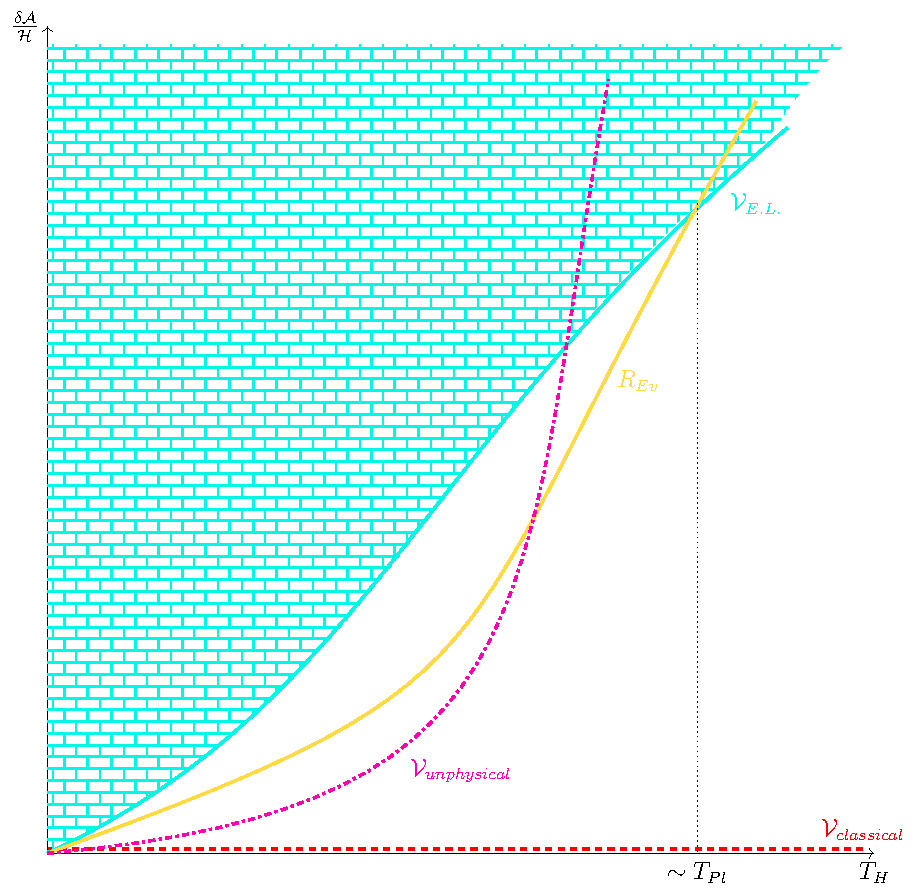
\includegraphics[scale=0.77]{Immagini/state-independent-bounds/state-independent-bounds.pdf}
	\caption[]{representation of the idea at the base of section \ref{subsec:state-independent-bounds}. We expect any physical bound to grow faster than the expected black hole evaporation rate, at least in the region \(T \lesssim T_{Pl}\). Energy conditions leading to bounds that do not share this feature would lead to similar problems as the classical area theorem; we therefore would try to rule out those energy conditions, believed unphysical.}
	\label{fig:state-independent-bounds}
\end{figure}

